%=================AVANCES Y PRUEBAS=================
% SENSORES DE PULSO

\section{Velocímetro}
Para poder determinar la velocidad en la que se mueve un dispositivo dentro de un vehículo se realizó la integración del API de google, la cual nos permite saber la ubicación del dispositivo. Para poder confiar el la implantación de dicho velocímetro, se realizó una comparativa con un aplicación comercial (Waze) y un velocímetro analógico de un vehículo.\\

En la figura \ref{fig:Tvelocidad} se muestra la tabla correspondiente a las muestras tomadas, mismas que se encuentran en Km/h. La figura muestra una gráfica en la cual se observa con mejor claridad las diferencias.





\begin{figure}[htbp!]
	\centering
	\fbox{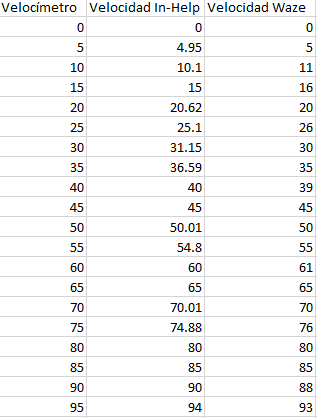
\includegraphics[width=.5\textwidth]{AvancesPruebas/imagenes/VelocimetroT}}
	\caption{Tabla comparativa medición de velocidades}
	\label{fig:Tvelocidad}
\end{figure}
\begin{figure}[htbp!]
	\centering
	\fbox{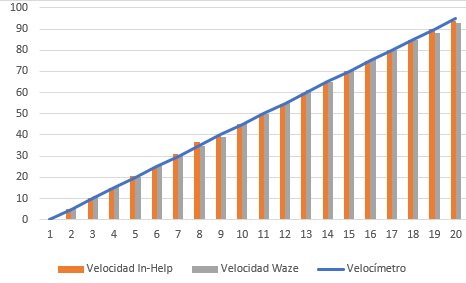
\includegraphics[width=.7\textwidth]{AvancesPruebas/imagenes/ValocidadWAI}}
	\caption{Gráfica comparativa medición de velocidades}
	\label{fig:GraficaWIA}
\end{figure}



 